



In this section, we analyze the trade-off between security, goodput, and latency achieved by various MAC schemes based on their tag sizes and tag-to-message ratios (TMR).
The tag-bits per message (TbpM) is a metric used to measure the integrity and availability of the system. Moreover, Goodput and TMR are metrics to show both the bandwidth and energy efficiency of the system.. 


\subsection{Computation and Latency Overhead}

To evaluate latency and computational overhead of different MAC schemes, we use an application-level metric based on real-time video streaming. Specifically, we measure the number of successfully verified frames per second (FPS) in our 5G experimental testbed, as shown in Fig.~\ref{fig:fps}. Since the camera generates frames at a fixed rate of 30 FPS, the achieved FPS reflects the system’s ability to process, authenticate, and verify packets in real time. Therefore, FPS serves as a practical proxy for both computational overhead and end-to-end latency.

\begin{figure}[h!]
	\centering
	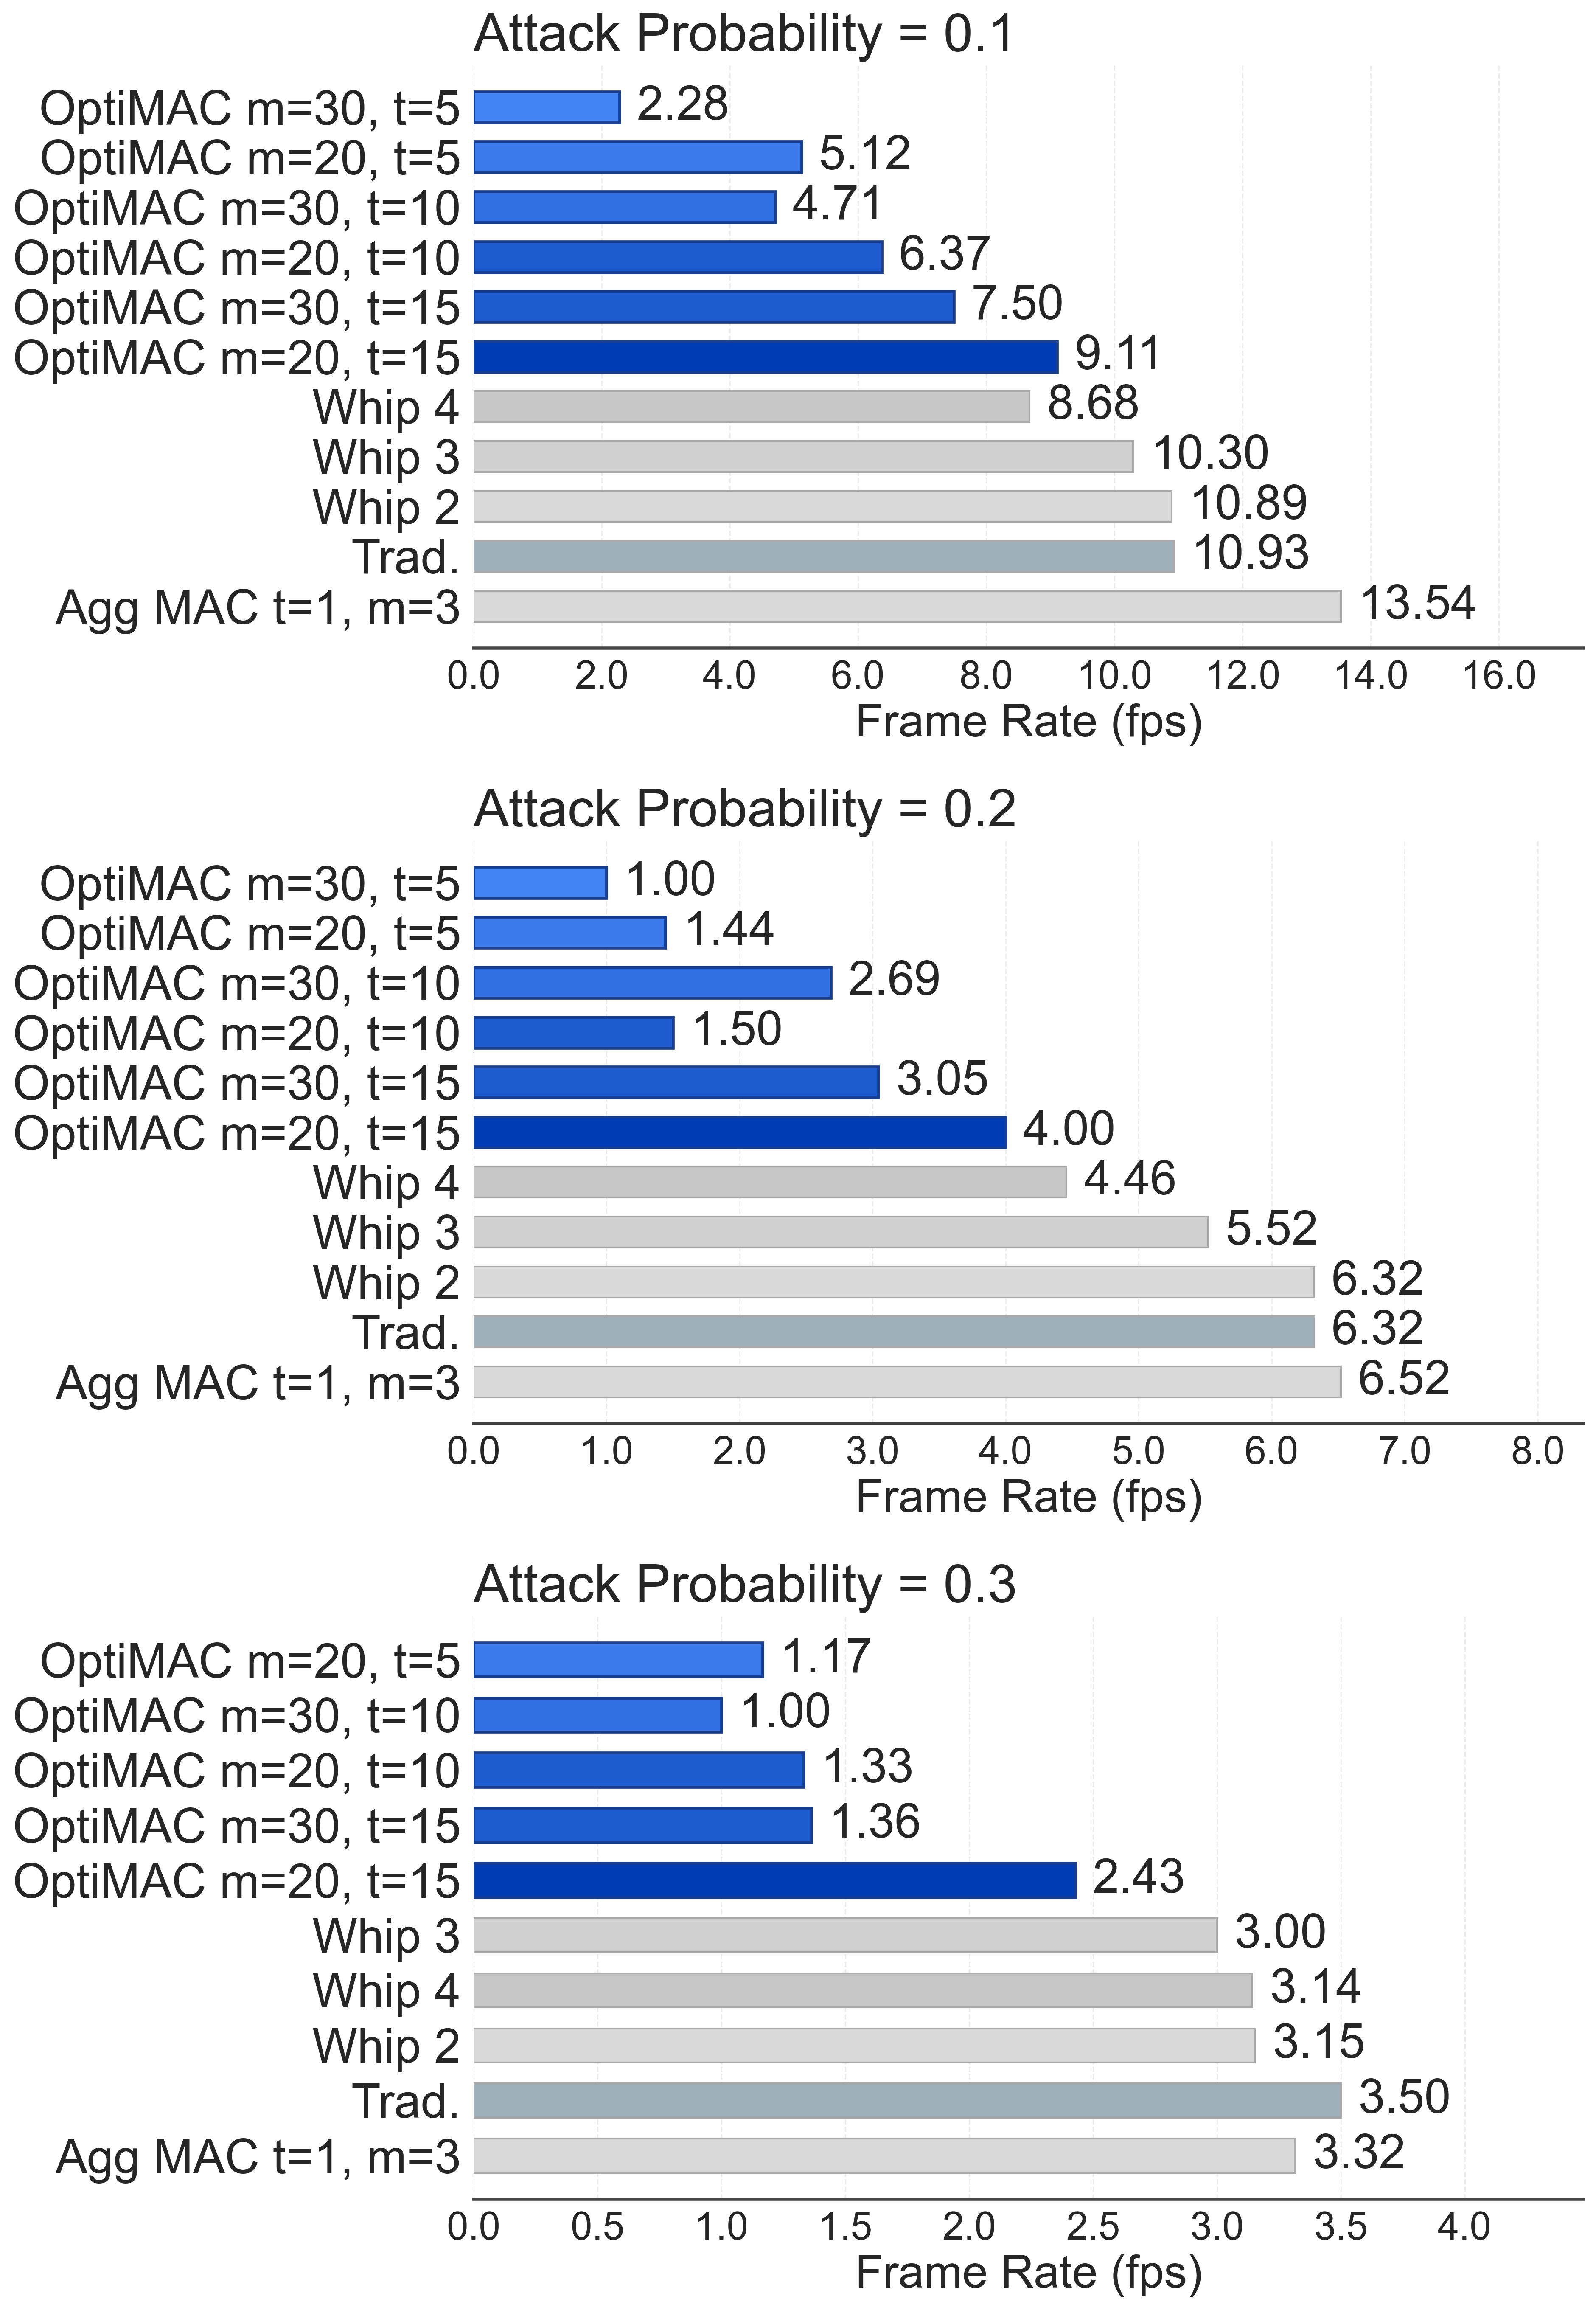
\includegraphics[width=\linewidth]{img/results/FrameRate.png}
	\caption{Frame rate (FPS)  under varying attack probabilities }
	\label{fig:fps}
\end{figure}

Fig.~\ref{fig:fps} shows the achieved frame rates under different attack probabilities (0.1, 0.2, and 0.3). As the attack probability increases, all schemes exhibit a reduction in FPS. This degradation is primarily due to increased packet loss, which limits the number of successfully verified packets available for frame reconstruction. In our implementation  correct decoding requires the availability of critical header and payload data. When a sufficient number of packets cannot be verified, the decoder fails to reconstruct the frame, resulting in dropped frames and a corresponding reduction in FPS. Furthermore, as the dependency matrix size increases, the authentication process becomes more complex, leading to higher authentication latency (L). This effect is evident when comparing different OptiMAC configurations, where smaller matrices (e.g., $t{=}10, m{=}20$) achieve higher FPS than larger ones (e.g., $t{=}15, m{=}30$) due to reduced verification delay. Therefore, the observed decrease in FPS reflects not only increased computational and communication overhead, but also the impact of both insufficient verified data and higher authentication latency under adversarial conditions.

Our prototype is implemented in Python at the application layer and is not optimized for performance. Nevertheless, OptiMAC supports real-time streaming at practical frame rates. A production-level implementation (e.g., in C/C++ or at the data link layer) is expected to further reduce overhead and latency. 

\subsection{Tag-bit per Message (TbpM) vs Goodput}
Similar to progressive MAC~\cite{ProMAC1}, adjusting the tag bits per message could be advantageous in balancing the overhead trade-off. A higher TbpM allows for shortening the tag length while satisfying the security requirements. However, in lossy channels, where the expected number of verifications is lower than in error-free channels, shortening the tag must be done carefully. 
\begin{wrapfigure}{l}{0.6\linewidth}
	\centering
	
\includegraphics[width=\linewidth]{img/results/WiFi/0.1SG.png}
	\caption{TbpM vs. Goodput for WiFi where a 256-bit tag was used (above 128 bits is considered as high security) under 0.1 attack rate.}
	\label{fig:explaing}
\end{wrapfigure}
For a MAC scheme to be considered secure, it must maintain a tag size of at least 64 bits, as per NIST standards~\cite{nist_64bits}. However, NIST emphasizes the actual tag length that may vary depending on the specific algorithm employed, and some applications, like IPsec, mandate a minimum of 128-bit tags without truncation to ensure robust security~\cite{nist_gcm_update}. Without loss of generality, In the rest of this paper, we assume more than 128 and 256 Tag-bits per Message (TbpM) are high security for WiFi and 5G, respectively.

In our study, any scheme with TMR exceeding the threshold set by the aggregate MAC scheme (i.e., one tag per two messages) is a high TMR scheme. Low TMR schemes are expected to offer more efficient bandwidth and computational usage by lowering the number of tags transmitted, though this may impact security if not managed carefully. By comparing various approaches in terms of security (measured in TbpM), we demonstrate the potential of optiMAC schemes to balance these factors, particularly in adversarial environments.

The results, visualized in Figure~\ref{fig:explaing}, illustrate that optiMAC (indicated in blue) generally outperforms state-of-the-art methods (in red) by achieving both high security and goodput.  The figure is divided into quadrants with shaded regions to indicate different trade-offs. The green area represents methods that achieve best in both metrics. The blue and light pink areas highlight methods that emphasize one metric but have sacrificed the other. The red area shows methods with both metrics are low, making these methods less desirable. By comparing the positions of red and blue points, it can be observed the relative performance of different methods. Blue points often appear in the green quadrant, suggesting a favorable balance between the metrics. 
%\begin{figure*}[h]
%     \centering
%          \begin{subfigure}[b]{0.32\linewidth}
%         \centering
%         
\includegraphics[width=\linewidth]{img/results/WiFi/0.1S'.png}
%         \caption{Attack rate 0.1}
%         \label{fig:0.1S WiFi}
%     \end{subfigure} \hfill
%     \begin{subfigure}[b]{0.32\linewidth}
%         \centering
%         
\includegraphics[width=\linewidth]{img/results/WiFi/0.2S'.png}
%         \caption{Attack rate 0.2}
%         \label{fig:0.2S WiFi}
%     \end{subfigure}
%     \hfill
%      \begin{subfigure}[b]{0.32\linewidth}
%         \centering
%         
\includegraphics[width=\linewidth]{img/results/WiFi/0.3S'.png}
%         \caption{Attack rate 0.3}
%         \label{fig:0.3S WiFi}
%     \end{subfigure}
%
%     \caption{TbpM (y-axis) vs. TMR (x-axis) of WiFi experiments with 256-bit tags (128 or higher TbpM is high security). State-of-the-art (SOTA) includes traditional, progressive, and aggregate MAC vs. the optimal by optiMAC.}
%     \label{fig:SecurityWiFi}
%\end{figure*}
%\begin{figure*}[h]
%     \centering
%          \begin{subfigure}[b]{0.32\linewidth}
%         \centering
%         
\includegraphics[width=\linewidth]{img/results/WiFi/0.1G'.png}
%         \caption{Attack rate 0.1}
%         \label{fig:0.1G WiFi}
%     \end{subfigure} \hfill
%     \begin{subfigure}[b]{0.32\linewidth}
%         \centering
%         
\includegraphics[width=\linewidth]{img/results/WiFi/0.2G'.png}
%         \caption{Attack rate 0.2}
%         \label{fig:0.2G WiFi}
%     \end{subfigure}
%     \hfill
%      \begin{subfigure}[b]{0.32\linewidth}
%         \centering
%         
\includegraphics[width=\linewidth]{img/results/WiFi/0.3G'.png}
%         \caption{Attack rate 0.3}
%         \label{fig:0.3G WiFi}
%     \end{subfigure}
%
%     \caption{Goodput (y-axis) vs. TMR (x-axis) of WiFi experiments where more than 80\% of Traditional MAC's Goodput is considered high. State-of-the-art (SOTA) includes traditional, progressive, and aggregate MAC vs. the optimal by optiMAC.}
%     \label{fig:GoodputWiFi}
%\end{figure*}
Each data point in the figure represents a specific method or configuration. Red points indicate state-of-the-art (SOTA) methods, while blue points represent the optiMAC model. The labels adjacent to the points (e.g., ProMAC and Agg MAC) correspond to different methods, and the accompanying values denote the tag-to-message ratio (TMR). For instance, a TMR of 0.9 implies that for every 10 messages, there are 9 tags, highlighting the balance between security and overhead. As shown in Figure~\ref{fig:explaing}, the Aggregate MAC achieves high security and the highest goodput. On the other hand, optiMAC offers enhanced security with only a slight reduction in goodput (Pareto optimal), demonstrating the trade-off between these factors. This flexibility allows our model to adapt to the specific requirements of various applications, even under adversarial scenarios.

\subsection{Security and Goodput vs TMR}

\begin{figure*}[h]
	\centering
	\begin{subfigure}[b]{0.32\linewidth}
		\centering
		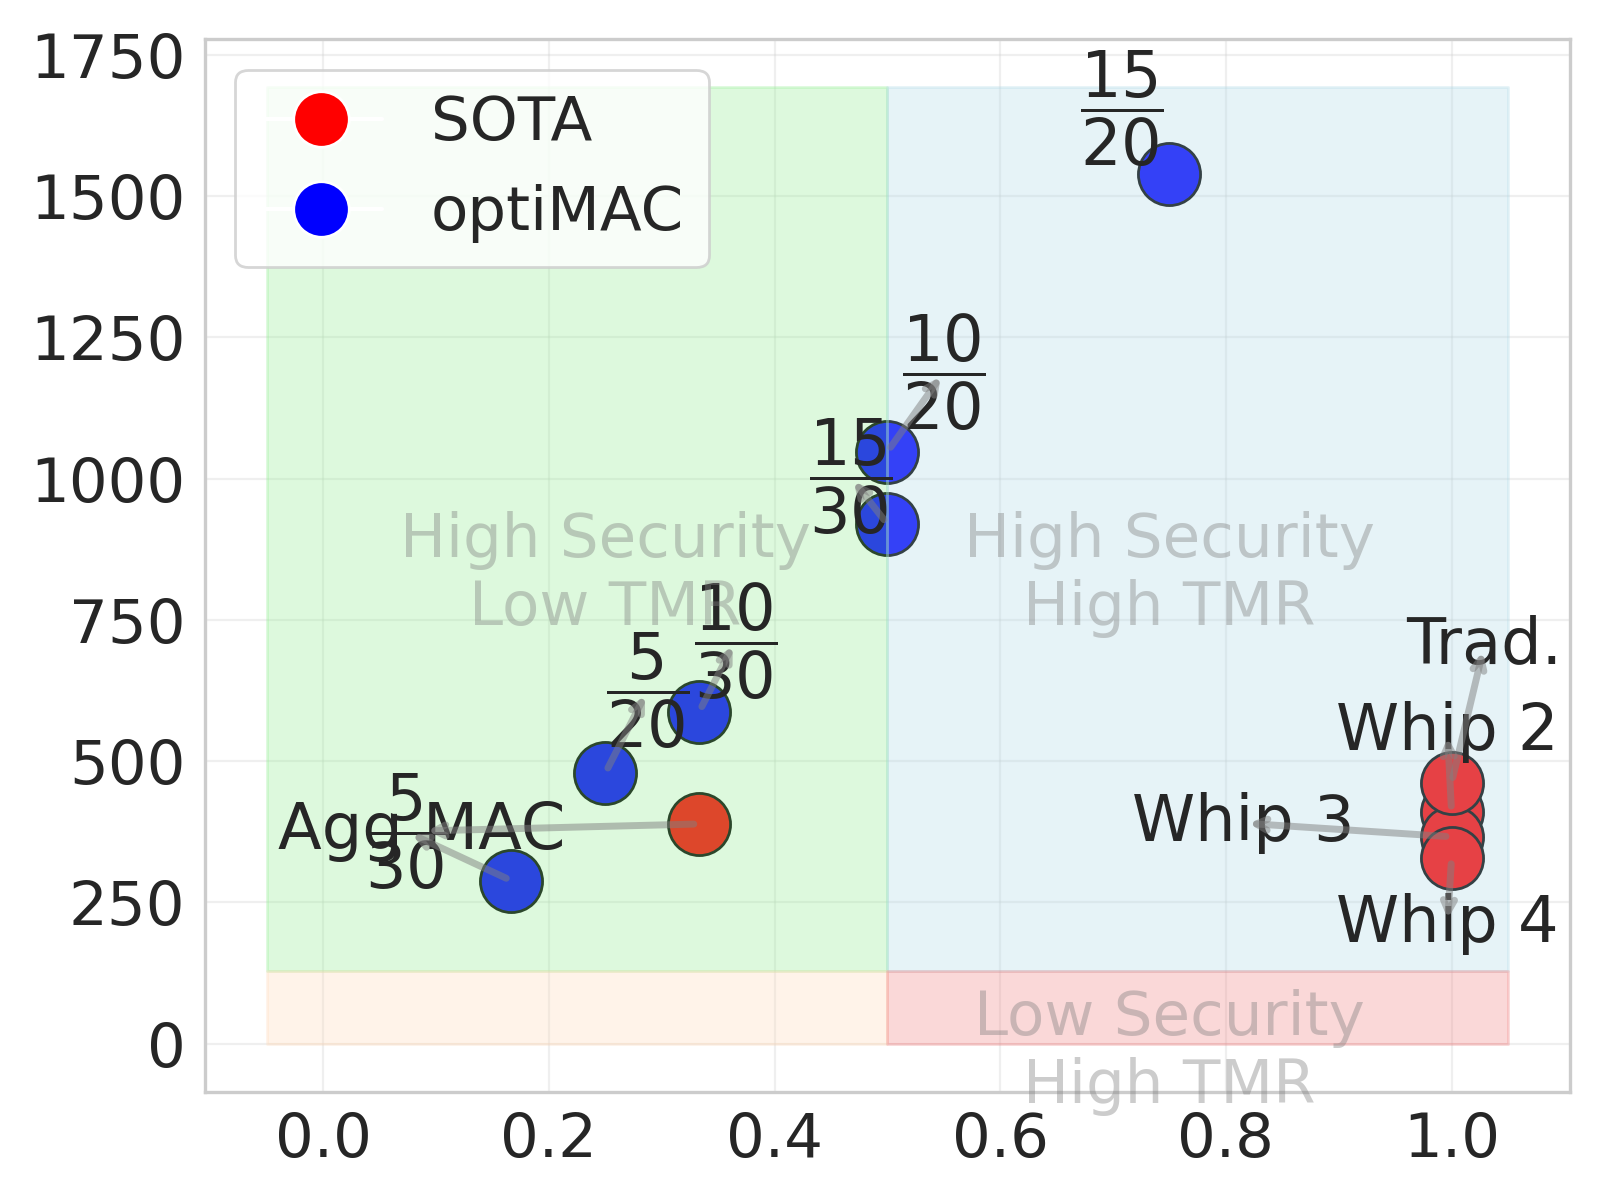
\includegraphics[width=\linewidth]{img/results/5G/0.1S'.png}
		\caption{Attack rate 0.1}
		\label{fig:0.1S 5G}
	\end{subfigure} \hfill
	\begin{subfigure}[b]{0.32\linewidth}
		\centering
		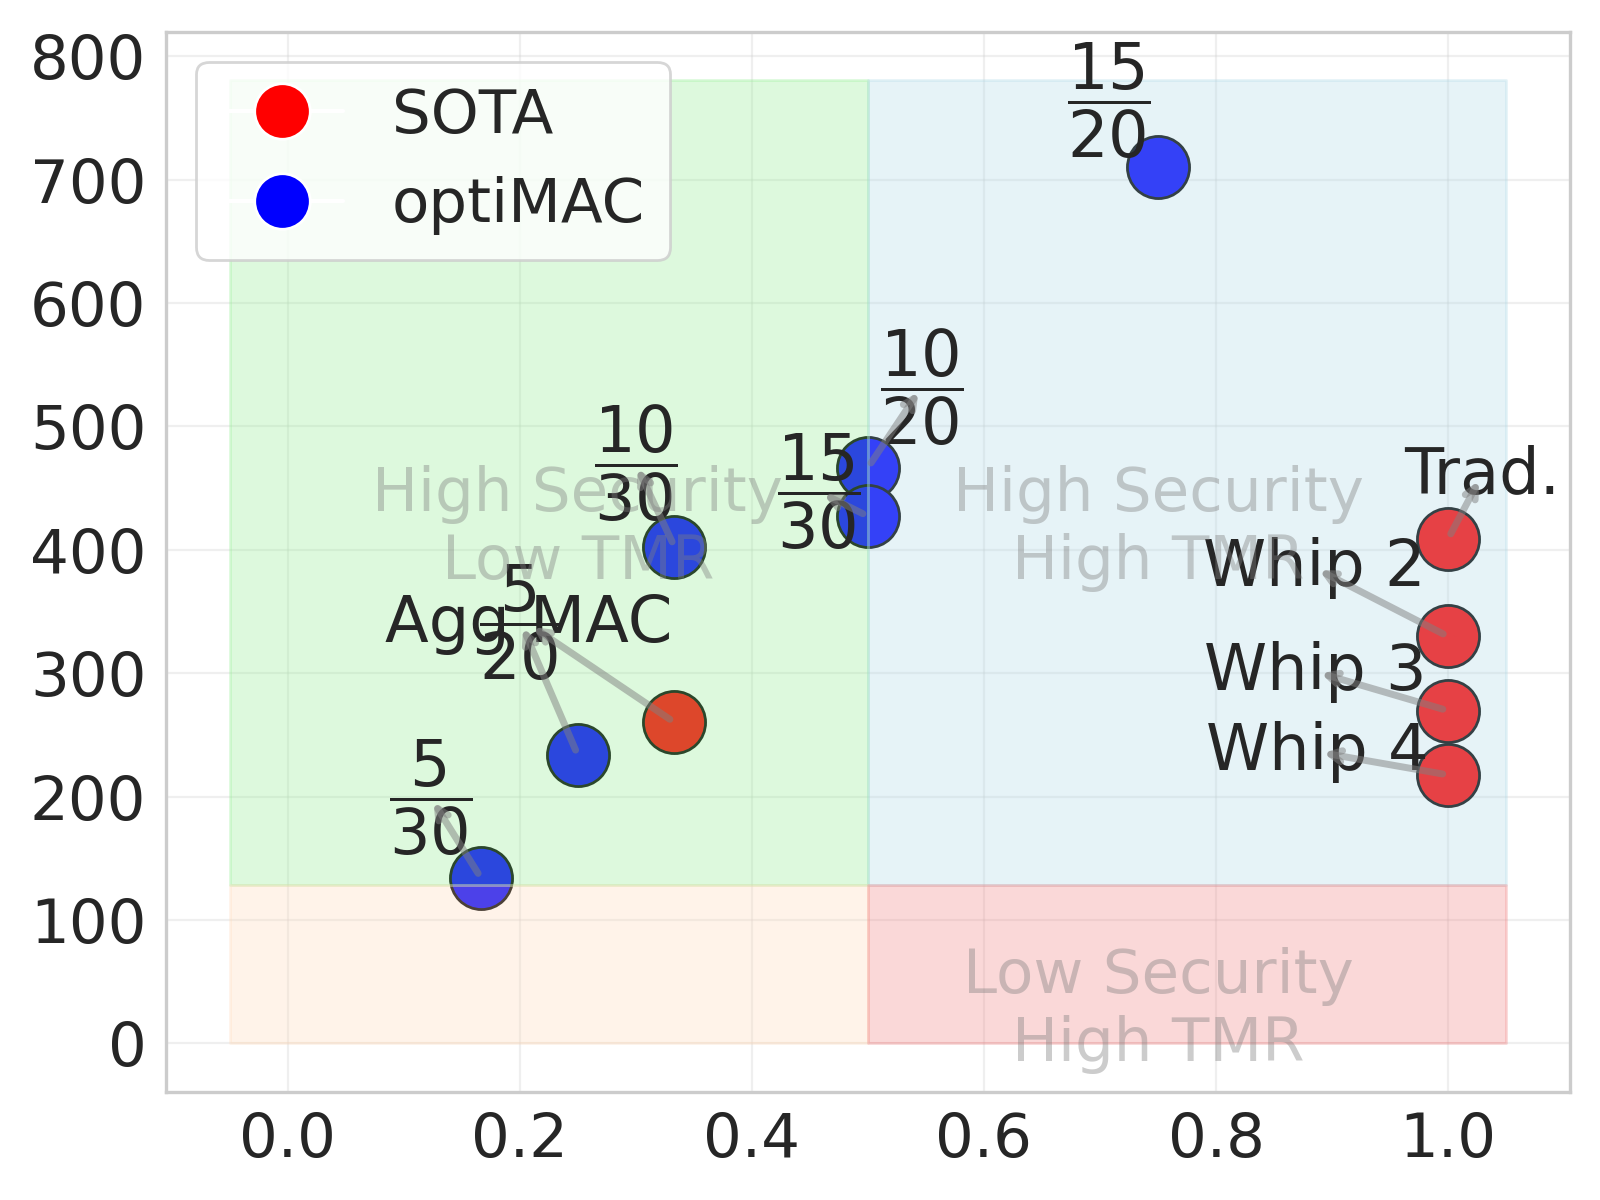
\includegraphics[width=\linewidth]{img/results/5G/0.2S'.png}
		\caption{Attack rate 0.2}
		\label{fig:0.2S 5G}
	\end{subfigure}
	\hfill
	\begin{subfigure}[b]{0.32\linewidth}
		\centering
		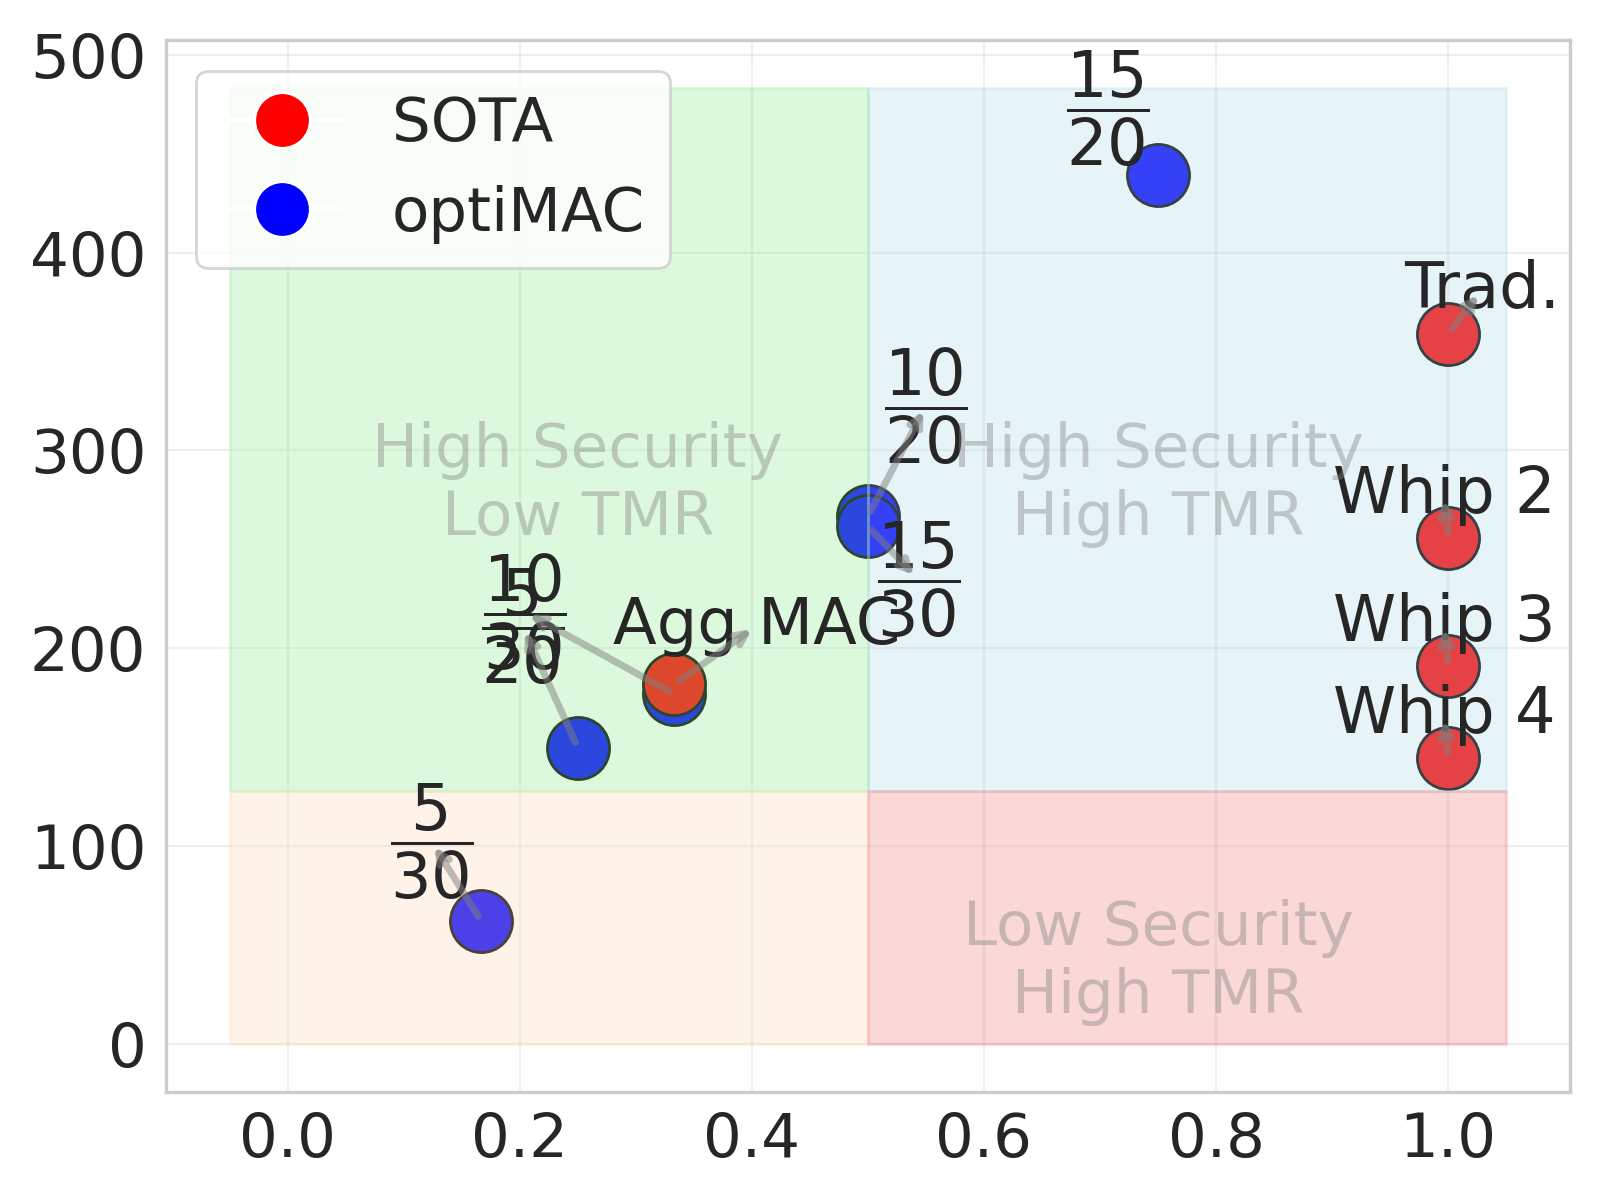
\includegraphics[width=\linewidth]{img/results/5G/0.3S'.png}
		\caption{Attack rate 0.3}
		\label{fig:0.3S 5G}
	\end{subfigure}
	
	\caption{TbpM (y-axis) vs. TMR (x-axis) of 5G experiments with 512-bit tags (256 or higher TbpM is high security). State-of-the-art (SOTA) includes traditional, progressive, and aggregate MAC vs. the optiMAC.}
	\label{fig:Security5G}
\end{figure*}

\begin{figure*}[h]
	\centering
	\begin{subfigure}[b]{0.32\linewidth}
		\centering
		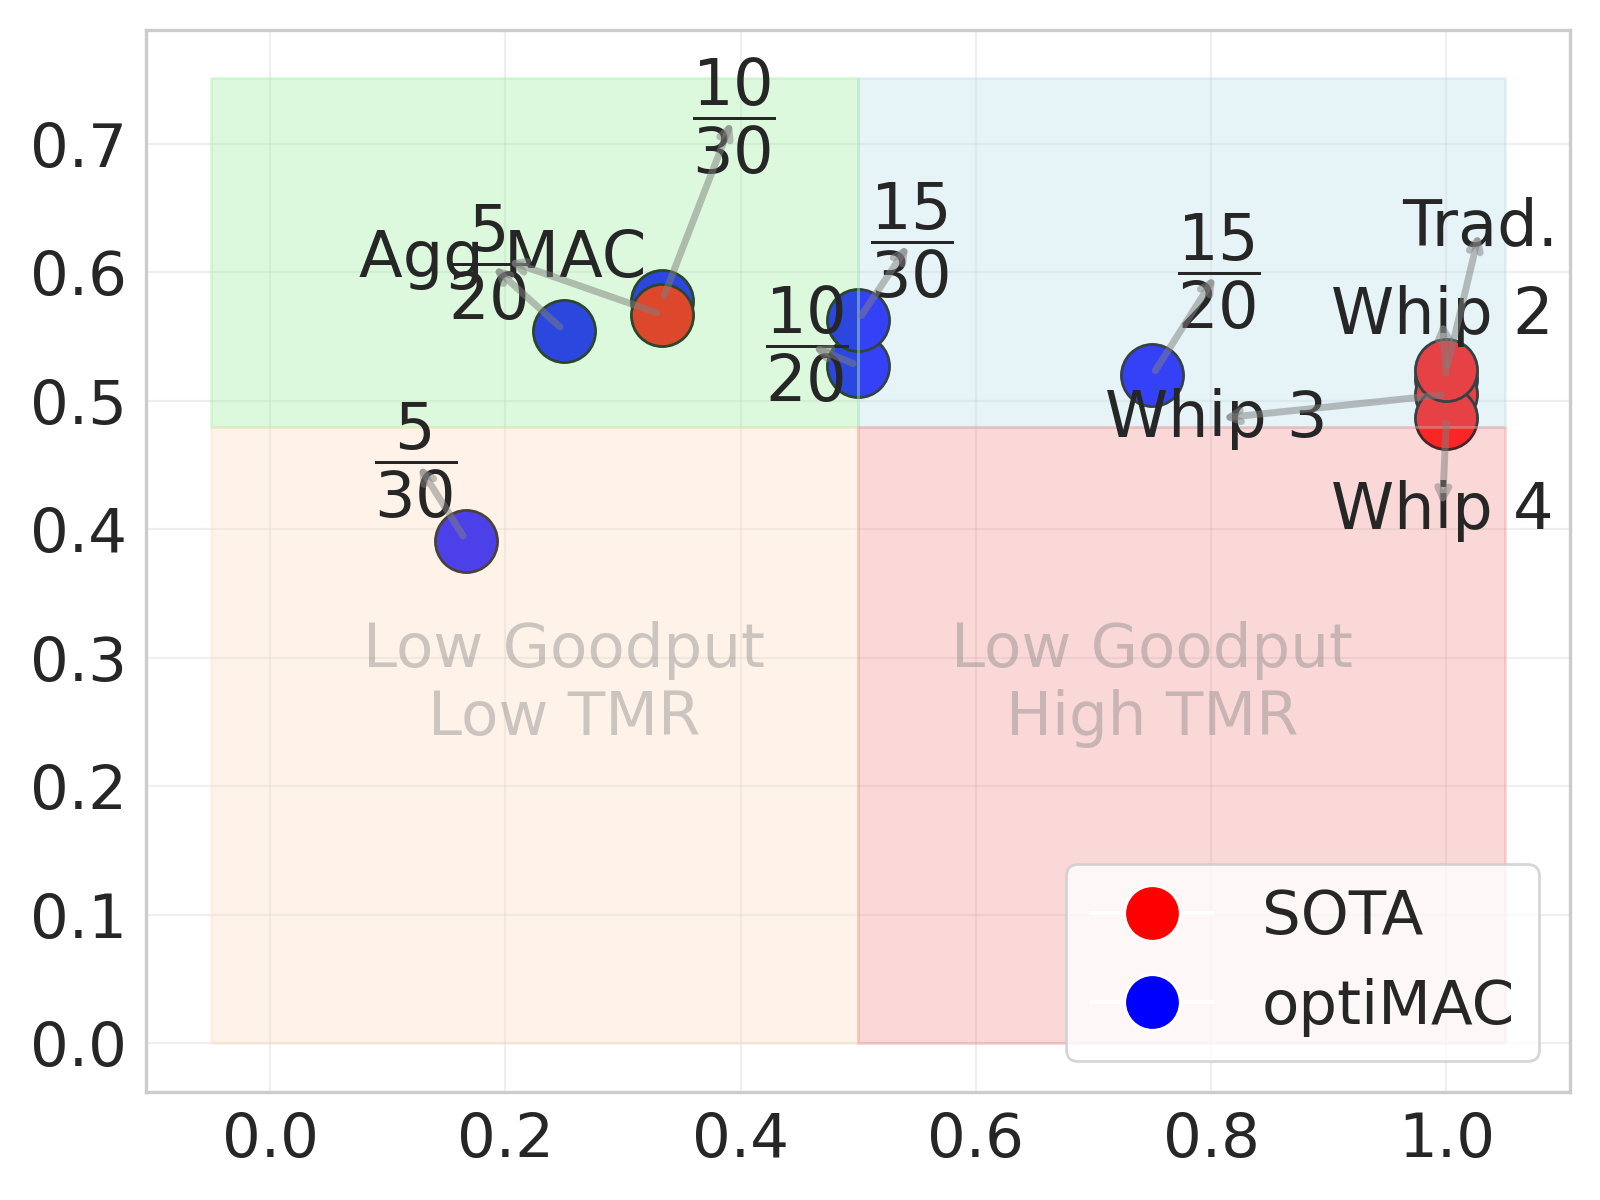
\includegraphics[width=\linewidth]{img/results/5G/0.1G'.png}
		\caption{Attack rate 0.1}
		\label{fig:0.1G 5G}
	\end{subfigure} \hfill
	\begin{subfigure}[b]{0.32\linewidth}
		\centering
		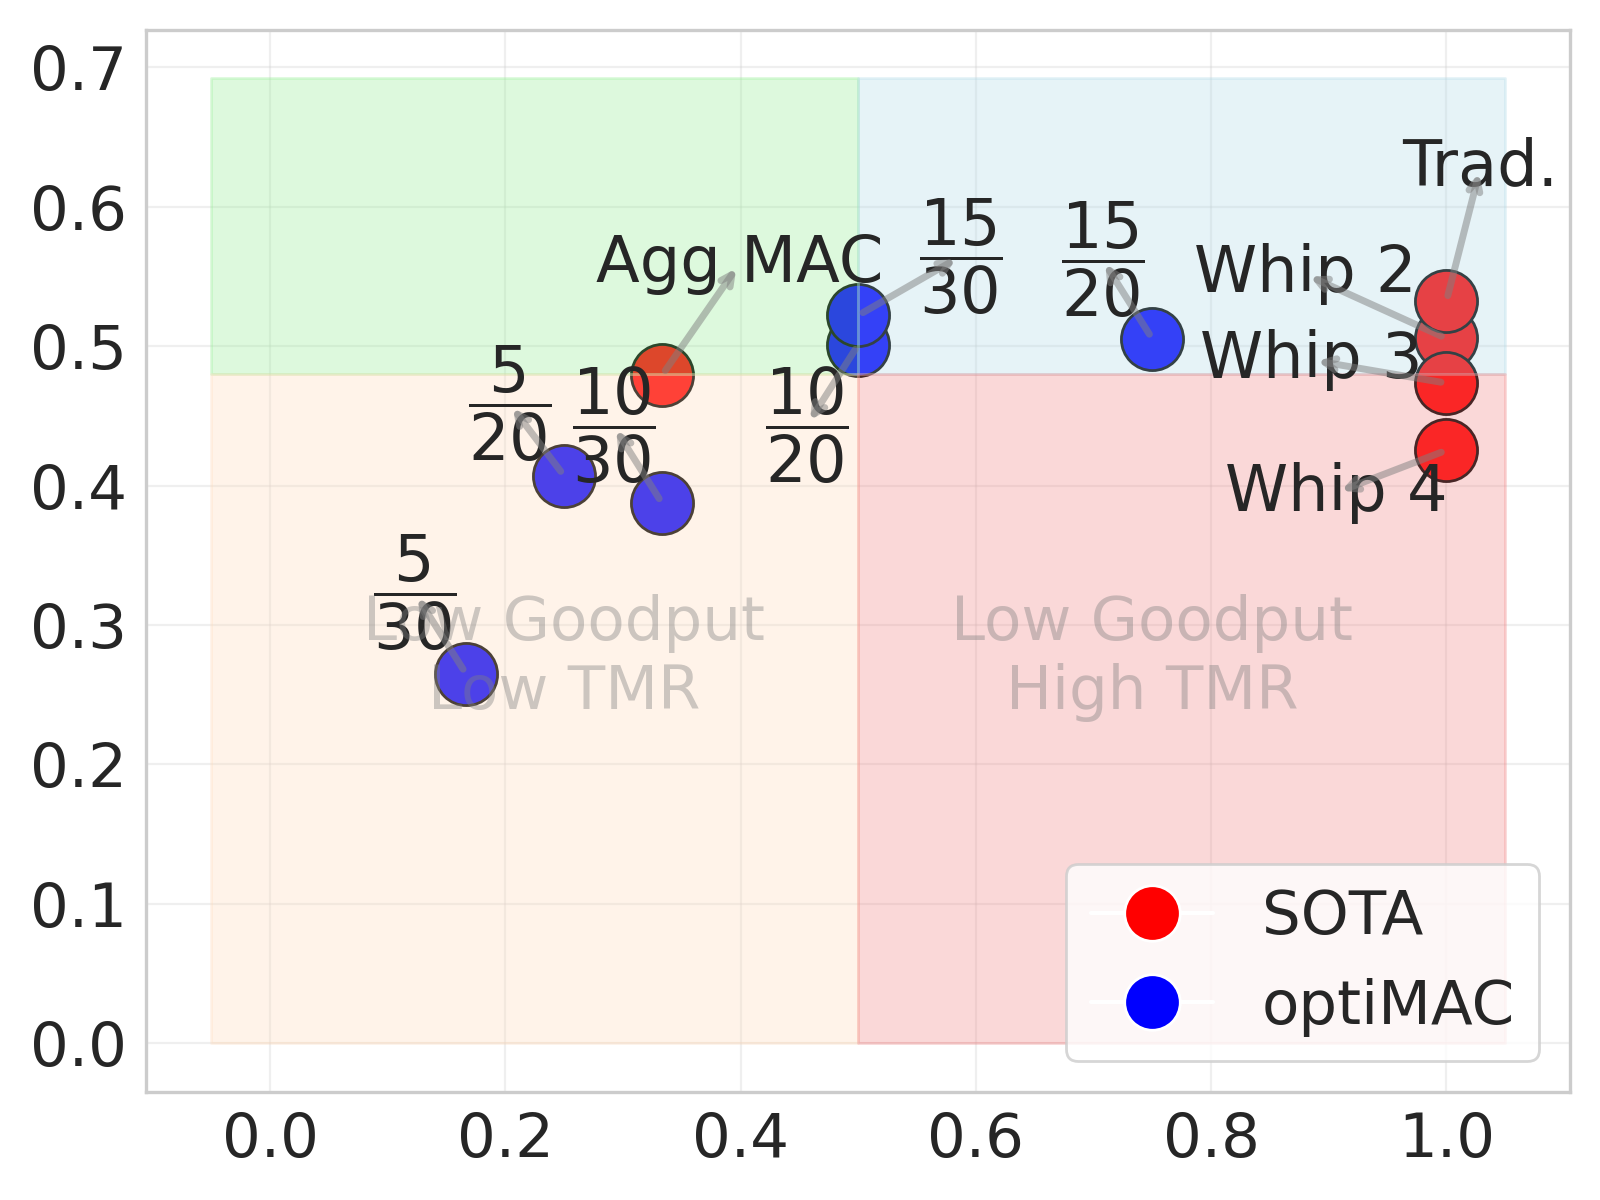
\includegraphics[width=\linewidth]{img/results/5G/0.2G'.png}
		\caption{Attack rate 0.2}
		\label{fig:0.2G 5G}
	\end{subfigure}
	\hfill
	\begin{subfigure}[b]{0.32\linewidth}
		\centering
		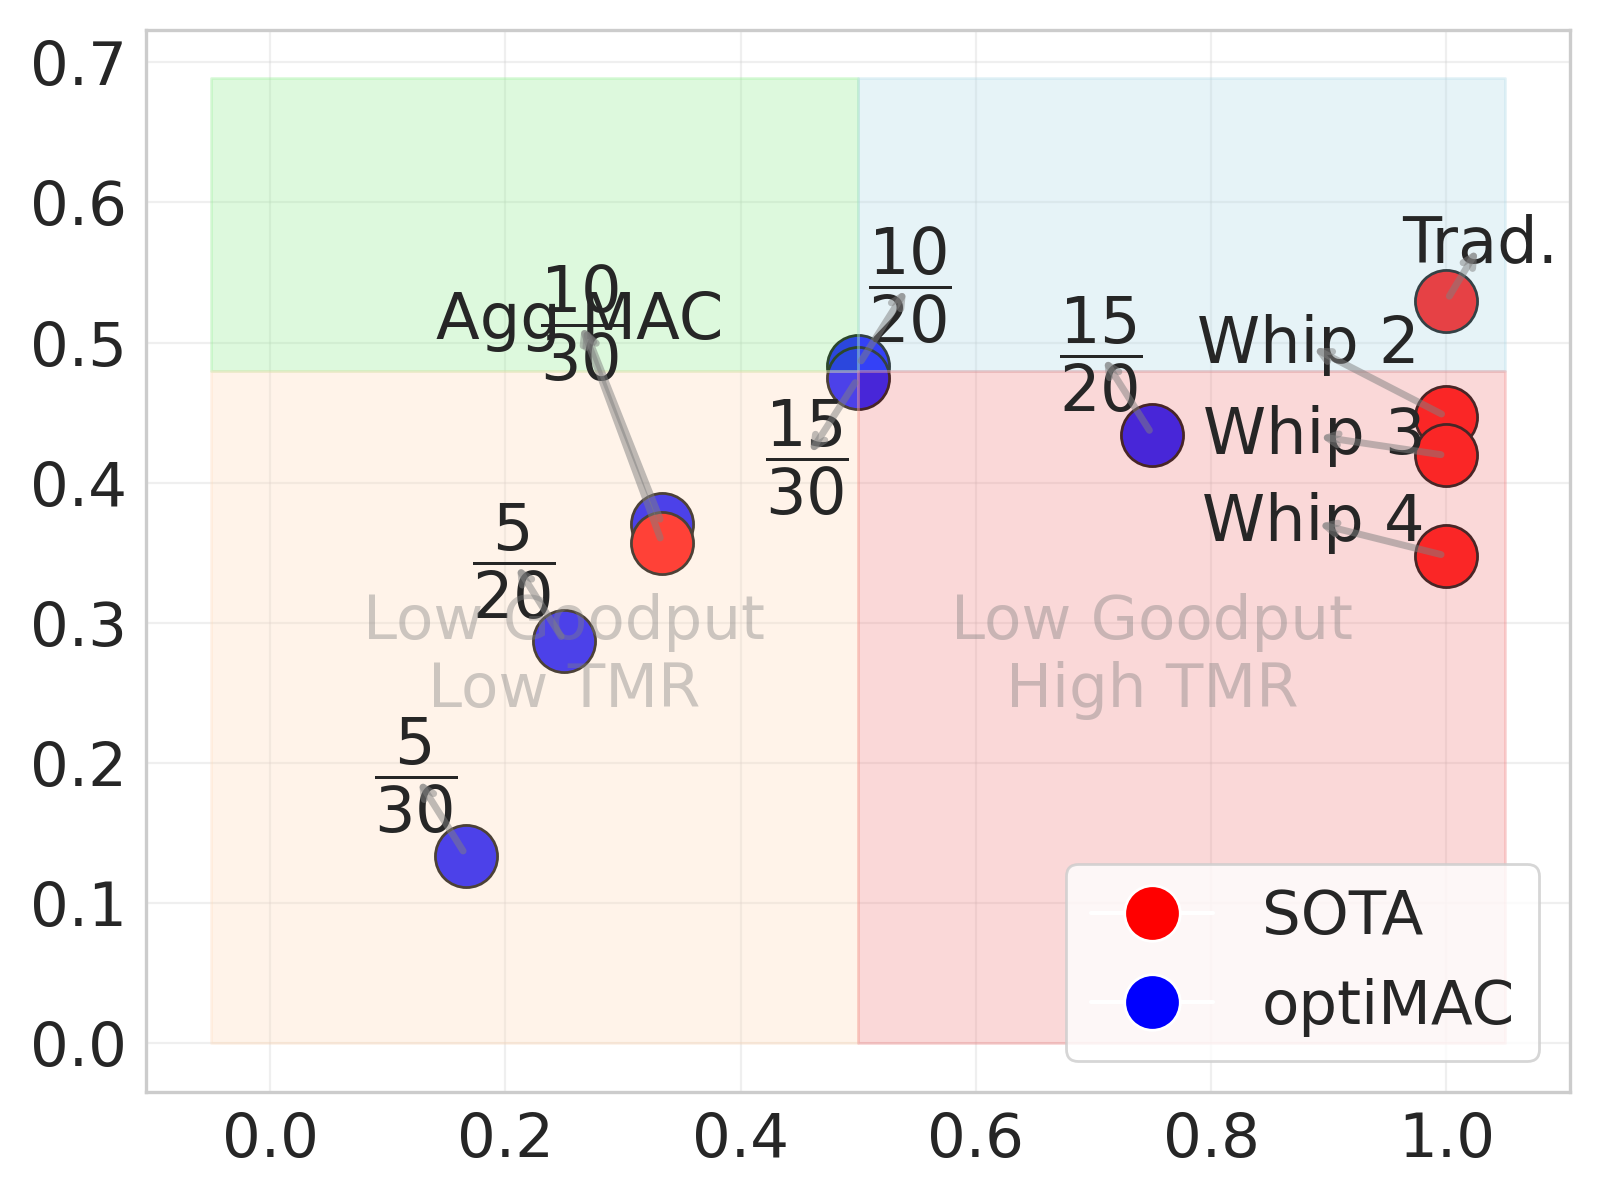
\includegraphics[width=\linewidth]{img/results/5G/0.3G'.png}
		\caption{Attack rate 0.3}
		\label{fig:0.3G 5G}
	\end{subfigure}
	
	\caption{Goodput (y-axis) vs. TMR (x-axis) of 5G experiments where more than 80\% of Traditional MAC's Goodput is considered high. State-of-the-art (SOTA) includes traditional, progressive, and aggregate MAC vs. the optiMAC.}
	\label{fig:goodput5G}
\end{figure*}

Figure~\ref{fig:Security5G} illustrates the performance of different MAC schemes (SOTA, OptiMAC, Agg. MAC, and various ProMAC versions) under varying attack rates (0.1, 0.2, and 0.3). Each subgraph plots the "Tag-bits per Message" (y-axis) against the "TMR" 
$\frac{n}{m}$ (x-axis), providing insights into the trade-offs between security and overhead.

We note that the WiFi results are not shown due to space limitations, as they exhibit trends nearly identical to the 5G results. Specifically, the relative performance ordering of the schemes, the security–overhead trade-offs, and the impact of increasing attack rates remain consistent across both network settings. Therefore, to avoid redundancy and improve clarity, we focus on presenting the 5G results, which are representative of both environments.

OptiMAC (depicted in blue) consistently achieves a balance between high security and low TMR, placing it in the "High Security, Low TMR" (green) region and satisfying Goal G2. It appears at lower tag-to-message ratios ($\frac{n}{m}$), indicating that it achieves strong security without requiring large redundancy, thereby reducing overhead. This demonstrates its efficiency compared to other schemes.

The SOTA solutions, shown in red, generally achieve high security but at higher TMR values, often placing them in the "High Security, High TMR" (blue) region, especially under higher attack rates. This indicates that while SOTA methods are effective, they incur significantly higher overhead compared to OptiMAC.

The Agg. MAC, when configured with a TMR of $\frac{1}{3}$, can achieve high security with low TMR under moderate attack rates, placing it in favorable regions of the plot. However, its performance degrades under higher attack rates (e.g., 0.3), where it transitions into the "Low Security, Low TMR" region, indicating insufficient robustness. In contrast, ProMAC variants (with dependency areas of 2, 3, and 4 without tag length adjustment) generally occupy the "Low Security, High TMR" or "High Security, High TMR" regions. While they can provide improved security over Agg. MAC, they do so at the cost of significantly increased overhead.

As the attack rate increases (from 0.1 to 0.3), all schemes exhibit a decrease in tag-bits per message, reflecting the need for increased redundancy to maintain security in more adversarial conditions.

Although not shown, the WiFi experiments follow the same trends, with differences in absolute values due to system parameters. In particular, WiFi exhibits lower tag-bits per message compared to 5G due to shorter tag lengths (32 vs. 64 bytes) and smaller payload sizes, as summarized in Table~\ref{tab:setting}.

Furthermore, by observing the trend of the OptiMAC configurations (blue points) in the goodput analysis (Figure~\ref{fig:goodput5G}), we identify a characteristic curve indicating an optimal operating region where goodput is maximized while maintaining required security levels (Goal G1). Selecting configurations near this peak enables an effective balance between security and efficiency under varying attack conditions.